\chapter{Cài đặt và thực nghiệm}
\section{Môi trường và checkpoint}
\begin{table}[H]
\centering
\caption{Cấu hình chạy. Điền môi trường benchmark thực tế.}
\begin{tabularx}{\textwidth}{@{}l L@{}}
\toprule
Thành phần & Cấu hình \\
\midrule
Checkpoint & \texttt{CIDAS/clipseg-rd64-refined} \\
Phiên bản / commit & [Điền từ run.json] \\
Thiết bị & [CPU / GPU và dung lượng VRAM] \\
Python, PyTorch, Transformers & [Điền phiên bản] \\
Seed và ngưỡng & [Điền cấu hình đã khóa] \\
\bottomrule
\end{tabularx}
\end{table}

\section{Dữ liệu và protocol}
[Ghi nguồn PhraseCut miniv, số ảnh/query thực tế, cách chọn tập con và tách calibration/evaluation theo image\_id. Tách bảng số liệu khác split hoặc protocol.]

\section{Độ đo đánh giá}
Gọi $I_i=|\hat{y}_i\cap y_i|$ và $U_i=|\hat{y}_i\cup y_i|$. Trung bình theo query và cumulative IoU được tính bằng:
\begin{equation}
\operatorname{meanIoU}=\frac{1}{N}\sum_{i=1}^{N}\frac{I_i}{U_i},\qquad
\operatorname{cIoU}=\frac{\sum_i I_i}{\sum_i U_i}.
\end{equation}
Dice được tính bằng $2|\hat{y}\cap y|/(|\hat{y}|+|y|)$. AP pixel được tính theo query rồi lấy trung bình trong code hiện tại. Cần ghi rõ protocol này khi so sánh với số bài báo.

\section{E1: Baseline text}
\begin{table}[H]
\centering
\caption{Khung kết quả E1. Dấu gạch ngang biểu thị chưa có số liệu.}
\label{tab:e1}
\begin{tabular}{@{}lccccc@{}}
\toprule
Cấu hình & $N$ & Ngưỡng & mean IoU & cIoU & AP \\
\midrule
Text baseline & --- & 0,3 & --- & --- & --- \\
Ngưỡng calibration & --- & --- & --- & --- & --- \\
\bottomrule
\end{tabular}
\end{table}
[Phân tích kết quả và giải thích khác biệt với số tham chiếu từ bài báo.]

\section{E2: Text so với visual prompt}
\begin{table}[H]
\centering
\caption{Khung kết quả E2 trên cùng tập query có support hợp lệ.}
\label{tab:e2}
\begin{tabular}{@{}lcccc@{}}
\toprule
Prompt & $N$ & mean IoU & cIoU & AP \\
\midrule
Text & --- & --- & --- & --- \\
Support crop & --- & --- & --- & --- \\
Support giảm nền & --- & --- & --- & --- \\
\bottomrule
\end{tabular}
\end{table}
[Bổ sung manifest support, ngưỡng và phân tích từng cặp query.]

\section{E3: Prompt engineering}
\begin{table}[H]
\centering
\caption{Khung kết quả E3. Giữ cùng ảnh, mục tiêu, GT và ngưỡng.}
\label{tab:e3}
\begin{tabularx}{\textwidth}{@{}Lccc@{}}
\toprule
Template & mean IoU & cIoU & AP \\
\midrule
\texttt{\{phrase\}} & --- & --- & --- \\
\texttt{a photo of \{phrase\}} & --- & --- & --- \\
\texttt{the \{phrase\}} & --- & --- & --- \\
\texttt{\{phrase\} in the image} & --- & --- & --- \\
\bottomrule
\end{tabularx}
\end{table}
[Phân tích template tốt và kém; không chọn template bằng tập evaluation rồi coi là đánh giá độc lập.]

\section{Phân tích lỗi và demo}
\begin{figure}[H]
\centering
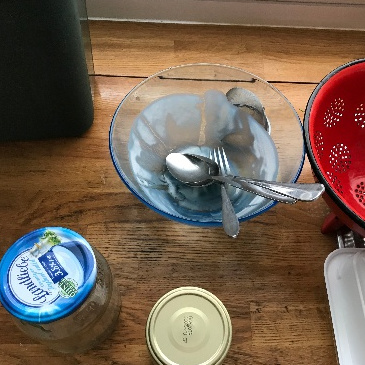
\includegraphics[width=0.31\textwidth]{demo_query.jpg}\hfill
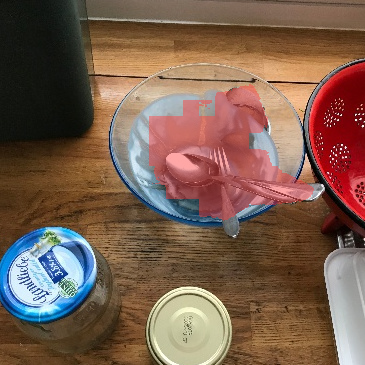
\includegraphics[width=0.31\textwidth]{demo_text.png}\hfill
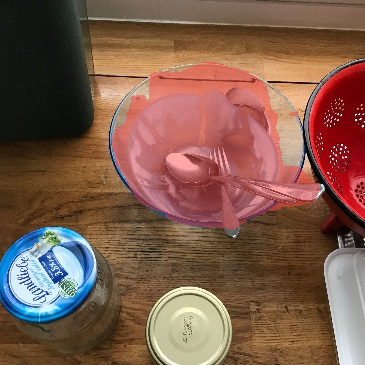
\includegraphics[width=0.31\textwidth]{demo_visual.png}
\caption{Kiểm tra inference ban đầu: ảnh query từ repo tác giả~\cite{clipsegcode}, text ``a spoon'' và visual crop cùng ảnh. Ví dụ này chưa có GT và không dùng làm kết quả E2.}
\label{fig:smoke}
\end{figure}
[Thay hoặc bổ sung các hình có GT để phân tích vật nhỏ, nhiều vật, thuộc tính và quan hệ.]
